\chapter{Modellierung Isolierte Ereignisse}

In diesem Kapitel soll ein Risikomodell f�r die Isolierten Ereignisse in der Phase regen Lebens (im Folgenden alternativ auch als Unf�lle bezeichnet) erstellt werden. Die Definition der Isolierten Ereignisse wird deshalb genauer analysiert, um die Anforderungen an das sp�tere Risikomodell abzuleiten. Es werden zwei Ans�tze vorgestellt, die diese Anforderungen erf�llen. Auf Basis von Krankenkassenabrechnungsdaten werden dann die Modellparameter f�r einen konkreten Anwendungsfall gesch�tzt und die Modellg�te bewertet.\\

\section{Grundlegende Betrachtungen}\label{sec:grundBet}

Im Kohorten-Modell werden die Unf�lle als \textbf{seltene Ereignisse}, welche die Gesundheit eines Versicherten beeintr�chtigen, \textbf{sich nicht ank�ndigen} und bei denen der Eintritts\-zeitpunkt der eigentliche \textbf{Ausl�ser von begrenzten Leistungsabfolgen} ist, beschrieben. Au�erdem sollen sie selten, und \textbf{unabh�ngig voneinander}, auftreten. Das hei�t die Eintrittswahrscheinlichkeit f�r einen Unfall h�ngt nicht davon ab, ob der Versicherte bereits einen Unfall hatte. Es gibt also insbesondere \textbf{keinen Lerneffekt} und \textbf{keine Folgesch�den} die im Modell ber�cksichtigt werden m�ssen. Au�erdem ist die durch den Unfall hervorgerufene Leistungsfolge begrenzt was bedeutet, dass \textbf{keine Chronizit�t} durch einen Unfall entstehen kann. Dadurch sind die isolierten Ereignisse klar zu den singul�ren Ereignisketten abgegrenzt, die im n�chsten Kapitel behandelt werden.\\

F�r das Kohorten-Modell m�ssen die isolierten Ereignisse in der Phase "`regen Lebens"' beschrieben werden. Deshalb werden f�r die Modellierung zwar alle Unf�lle hinzugezogen, aber die Kosten von Unf�llen aus den anderen beiden Phasen werden als jeweilige Phasen-Leistungen in der Krankenversicherungsbiographie kumuliert. Das hei�t insbesondere, dass Unf�lle mit Todesfolge keine besondere Betrachtung mehr ben�tigen, da sie bereits in der dritten Phase des Modells erfasst wurden.\\

Die Erfahrung zeigt, dass die Unfallwahrscheinlichkeit sowohl vom Alter als auch vom Geschlecht des Versicherten abh�ngen kann. Dabei ist zu beachten, dass es vom Unfalltyp abh�ngen wird, ob ein Zusammenhang besteht und wie stark dieser Zusammenhang ist. Des Weiteren k�nnen bestimmte Unf�lle auch von der Saison abh�ngen und so zum Beispiel h�ufiger im Winter auftreten als im Sommer.\\

Zusammenfassend l�sst sich sagen, dass die zu modellierende Unfallwahrscheinlichkeit unabh�ngig von bereits eingetretenen Unf�llen ist, aber, je nach Unfalltyp, vom Alter und Geschlecht des Versicherten abh�ngen und einer Saisonalit�t unterliegen kann. F�r die Modellierung werden wir die Saisonalit�t allerdings nicht besonders betrachten, da aufgrund des in der Regel sehr langen Beobachtungszeitraums, in der Phase regen Lebens, diese Effekte nur einen sehr geringen Einfluss auf das Modell haben werden. Auf Basis dieser Erkenntnisse werden nun zwei Modelle vorgestellt:

\section{Modell - Poisson-Prozess}
Die erwartenden Kosten f�r Unf�lle in der Phase regen Lebens, setzen sich aus zwei Teilen zusammen. Zum einen m�ssen die Kosten f�r einen Unfall modelliert werden und zum anderen ben�tigen wir einen Stochastischen Prozess, der die H�ufigkeit f�r einen Unfall in dem beobachteten Zeitraum z�hlt. Wir werden zuerst den Stochastischen Prozess betrachten. Eine Modellannahme ist, dass die Wahrscheinlichkeit f�r einen Unfall unabh�ngig davon ist, wann der vorherige Unfall eingetreten ist. Das hei�t der Stochastische Prozess hat unabh�ngige Zuw�chse. Au�erdem wird angenommen, dass aufgrund des Charakters der Unf�lle als seltene Ereignisse, die Genesungsdauer vernachl�ssigt werden kann. Das hei�t die begrenzte Leistungsfolge, die bei jeden Unfall ausgel�st wird, wird auf den Zeitpunkt des Unfalls konzentriert und die Zeit zwischen zwei Unf�llen, h�ngt nur von der Unfallwahrscheinlichkeit ab. Bevor wir den Prozess n�her beschreiben, f�hren wir folgende Bezeichnungen ein:

\begin{enumerate}[label=(\roman{*})]
	\item Die Unfallwahrscheinlichkeit wird mit $\lambda$ bezeichnet.
	\item Die Unfallzeitpunkte seien gegeben durch $t_1, t_2, t_3,...$ und weiterhin sei $t_0 = 0$ der Beginn der Beobachtung.
	\item Die Zeit zwischen den einzelnen Unf�llen sei definiert als $\{T_k\}_{k \geq 1}$ mit $T_k := t_k-t_{k-1}$.
	\item Die kumulierten Zwischenankunftszeiten werden mit $S_n = \sum_{k=1}^n T_k$ bezeichnet.
	\item Die Anzahl der Unf�lle wird bezeichnet durch 
	\begin{eqnarray*}
		N_t := max\{k : t_k \leq t\} = \sum_{k=1}^{\infty} \mathds{1}(S_k\leq t).
	\end{eqnarray*}
\end{enumerate}

Es ist leicht zu erkennen, dass $\{N_t, t\geq 0\}$ der gesuchte stochastische Prozess ist und gem�� Definition \ref{def:zaehlPro} ein Z�hlprozess ist. Laut Voraussetzung h�ngt die Unfallwahrscheinlichkeit nur vom Alter und Geschlecht der Versicherten ab. Ohne Einschr�nkung der Allgemeinheit k�nnen wir das Alter eines Versicherten als die Differenz aus dem aktuellen Jahr und seinem Geburtsjahr definieren. Das hei�t alle Versicherten werden immer zum 1.1. ein Jahr �lter. Da aufgrund der Modellannahmen keine weiteren Einflussfaktoren ber�cksichtigt werden m�ssen, ist somit die Unfallwahrscheinlichkeit eines Versicherten innerhalb eines Kalenderjahres konstant und die Unfallzeitpunkte sind gleichm��ig verteilt. Dann gilt f�r die Zwischenankunftszeiten $\{T_k\}_{k \geq 1}$, dass die Zeit bis zum n�chsten Unfall unabh�ngig davon ist, wie viel Zeit $s\geq 0$ bereits ohne einen Unfall verstrichen ist

\begin{eqnarray*}
	\mathbb(T_k>x+s | T_k>s) = \mathbb(T_k>x).
\end{eqnarray*}

Das hei�t die Verteilung der Zwischenankunftszeiten sind ged�chtnislos und somit gilt, gem�� Lemma \ref{lem:expLemma}, $T_k \sim exp(\lambda)$ f�r alle $k \geq 1$. Damit ist, innerhalb eines Kalenderjahres, $\{N_t, t\geq 0\}$, laut Definition \ref{def:poiPro}, ein homogener Poisson-Prozess und $N_t \sim Poi(\lambda t)$. Da ein Poisson-Prozess, gem�� Theorem \ref{th:poiPro} unabh�ngige und station�re Zuw�chse besitzt, passt dieser auch zu den eingangs aufgestellten Modellannahmen. An dieser Stelle sollte auch erw�hnt werden, dass aufgrund von Lemma \ref{lem:wartezeit} der Zeitpunkt, zu dem die Beobachtung beginnt, keinen Einfluss auf den Zeitpunkt des n�chsten beobachteten Unfalls hat. Deshalb ist auch die Zerlegung des Beobachtungszeitraumes in Jahresscheiben gerechtfertigt und die Summe der Unf�lle in den einzelnen Jahresscheiben ergibt dann die Anzahl an Unf�lle im Beobachtungszeitraum.\\

Als N�chstes m�ssen wir uns �berlegen, wie wir die Wahrscheinlichkeit f�r einen Unfall sch�tzen k�nnen. Da der Poisson-Prozess station�re Zuw�chse hat, k�nnen wir die Parameter auf Basis von historischen Informationen sch�tzen. Aufgrund der erwarteten Abh�ngigkeit von Alter und Geschlecht, muss f�r jede Kombination aus Altersgruppe und Geschlecht ein separates $\lambda_{Altersgruppe, Geschlecht}$ gesch�tzt werden. Dazu betrachten wir die relative H�ufigkeit eines Unfalls f�r die jeweilige Kombination aus Alter und Geschlecht und setzen
\begin{eqnarray} \label{eq:unfallWs}
	\bar{\lambda}_{Altersgruppe, Geschlecht} := \frac{\#\{\text{Unf�lle}\}_{Altersgruppe, Geschlecht}}{\#\{\text{Versicherte}\}_{Altersgruppe, Geschlecht}}.
\end{eqnarray}

Dabei ist $\#\{\text{Versicherte}\}_{Altersgruppe, Geschlecht}$ die Anzahl aller Versicherten, die in die jeweilige Alters- und Geschlechtsgruppe fallen und in dem betrachteten Zeitraum bei der Kasse versichert waren. Des Weiteren ist $\#\{\text{Unf�lle}\}_{Altersgruppe, Geschlecht}$ die Anzahl der Unf�lle, im betrachteten Zeitraum, von Personen, die in die jeweilige Alters- und Geschlechtsgruppe fallen. Es werden dabei alle F�lle betrachtet, die in dem jeweiligen Kalenderjahr begonnen haben, da wir Unf�lle auf den Eintrittszeitpunkt konzentrieren. Die Einteilung der Altersgruppen ist dabei flexibel. \\

Bisher haben wir nur die allgemeine Wahrscheinlichkeit f�r einen Unfall untersucht. Wie bereits am Anfang erw�hnt ist es sinnvoll verschiedene Unfalltypen zu betrachten, da sich diese hinsichtlich ihrer Kosten sehr stark unterscheiden k�nnen. Das Lemma \ref{lem:aufteilungPP} erlaubt es uns, den allgemeinen Unfall Prozess als eine �berlagerung von Teilprozessen darzustellen. Seien $U_1, U_2,...,U_n$ mit $n\in \mathbb{N}$ die verschiedenen, relevanten Unfalltypen und $\lambda _{U_1},\lambda _{U_2},...,\lambda _{U_n}$ die zugeh�rigen Unfallwahrscheinlichkeiten, dann gilt f�r die daraus resultierenden Prozesse 
\begin{eqnarray*} 
	N_t^{\lambda _{U_i}} &\sim& Poi(\lambda _{U_i} t) \\
	N_t^{\lambda} &:=& \sum^n_{i=1} N_t^{\lambda _{U_i}} \\
	N_t^{\lambda} &\sim& Poi(\sum_{i=0}^n\lambda _{U_i} t)
\end{eqnarray*}
Das hei�t der Prozess l�sst sich bei Bedarf beliebig in Unterprozesse zerlegen, die jeweils eine Teilmenge der Unf�lle beschreiben. Die Voraussetzung daf�r ist, dass die $N_{\lambda _{U_i}}$ unabh�ngig voneinander sind. Deshalb m�ssen die einzelnen Unfalltypen so abgrenzt werden, dass es nicht zu �berschneidungen kommt.\\

Damit ist der erste Teil der Modellierung abgeschlossen und wir k�nnen nun die Kosten betrachten. F�r jeden Unfalltyp sind diese aufgrund der Modellannahmen unabh�ngige und gleich verteilte Zufallsgr��en $X_1,X_2,...$, wobei $X_i$ die Kosten f�r den $i$-ten Unfall angibt. Bei Leistungskosten in der Krankenversicherung ist zu beobachten, dass es viele F�lle mit niedrigen Kosten und einige mit sehr hohen Kosten (Hochkostenf�llen) gibt, aber nur einen sehr geringen Teil mit durchschnittlichen Kosten. Aus diesem Grund ist es wichtig eine Verteilungsfunktion f�r die $\{X_i\}_{i>0}$ zu w�hlen, die zum einen die Standardf�lle abdeckt und zum anderen noch genug Masse in den hohen Kostenbereichen hat, um die Hochkostenf�lle nicht zu vernachl�ssigen. Verteilungsfunktionen mit dieser Eigenschaft werden auch als Heavy-Tail-Verteilung\footnote{z.B. Weibull-Verteilung mit Formparameter<1 oder Log-Normalverteilung} bezeichnet. Alternativ k�nnte als N�herung f�r die Kostenverteilung auch die empirische Verteilung auf Basis der historischen Informationen verwendet werden. Dabei werden die Kosten f�r alle Leistungen, die aus dem Unfall resultieren, zusammenaddiert, auch wenn die Leistungszeitpunkte weit auseinander liegen oder sogar in verschiedene Jahre fallen.\\

Bei der Modellierung der Leistungskosten ist au�erdem zu beachten, dass diese einer kontinuierlichen Ver�nderung, durch Preisver�nderungen oder die Einf�hrung alternativer Behandlungsmethoden, unterliegen. Es ist kann versucht werden, dies durch j�hrliche �nderungsraten auszugleichen, trotzdem sind in der Regel nicht genug Information vorhanden, um alle Einfl�sse auf die Kostenentwicklung zu ber�cksichtigen. Das optimale Vorgehen bei der Modellierung der Kostenverteilung h�ngt letztendlich vom Unfalltyp ab.\\ 

Kombinieren wir jetzt diese beiden Modellbestandteile, dann erhalten wir einen zusammengesetzten Poisson-Prozess, der die zuk�nftigen Kosten aufgrund von Unf�llen beschreibt. Dieser ist f�r jeden Unfalltyp $U$ definiert durch
\begin{eqnarray*} 
	Y_t^U = \sum_{i=1}^{N_t^U} X_i^U. 
\end{eqnarray*}
Das Risiko�quivalent, f�r die singul�ren Ereignisse eines Versicherten zum Zeitpunkt der Berechnung, entspricht somit der Summe der Barwerte\footnote{Der Barwert ist der Wert, den eine zuk�nftige Zahlung in der Gegenwart besitzt.}, der f�r die Phase regen Lebens vorhergesagten Unfallkosten.\\

Im weiteren Verlauf dieses Kapitels werden wir diesen Modellansatz beispielhaft f�r einen Unfalltyp implementieren und auswerten. Allerdings wird vorher noch ein alternativer Modellansatz vorgestellt, mit dem Unf�lle beschrieben werden k�nnen. 

\section{Alternativer Modellansatz - Markov-Kette}

Ein alternativer Modellansatz f�r die isolierten Ereignisse, kann mit Hilfe von Markov-Ketten konstruiert werden. Im Gegensatz zum Poisson-Ansatz k�nnen wir mit einer Markov-Kette die Genesungszeiten abbilden. Dadurch kann ausgeschlossen werden, dass ein Patient der im Krankenhaus behandelt wird in dieser Zeit einen weiteren Unfall erleidet. Ansonsten gelten weiterhin die unter \ref{sec:grundBet} beschriebenen Grundannahmen.  Wie bereits in Abschnitt \ref{sec:markov} gezeigt wurde, ist eine Markov-Kette durch ihre �bergangsmatrix eindeutig definiert. Deshalb werden wir beschreiben wie die Zust�nde und �bergangswahrscheinlichkeiten modelliert werden k�nnen. \\

Der Zustandsraum besteht im einfachsten Fall aus zwei Zust�nden: $i_0 :=$ Patient ist gesund und $i_1 :=$ Patient erholt sich von einem Unfall. Als Zeitraum f�r einen Prozessschritt bietet sich dabei ein Tag an, da Informationen zum Unfallzeitpunkt und zur Genesungsdauer in der Regel nur auf den Tag genau vorliegen. Die folgende Grafik veranschaulicht die m�glichen �berg�nge.\\

\begin{figure}[htb]
\centering
	\begin{tikzpicture}[->, >=stealth', auto, semithick, node distance=3cm]
	\tikzstyle{every state}=[fill=white,draw=black,thick,text=black,scale=1]
	\node[state]    (A)                     {$i_0$};
	\node[state]    (B)[right of=A]   {$i_1$};
	\path
	(A) edge[loop left]     node{$p_{0,0}$}         (A)
			edge[bend left,above]      node{$p_{0,1}$}      (B)
	(B) edge[loop right]    node{$p_{1,1}$}     (B)
			edge[bend left,below]    node{$p_{1,0}$}      (A);
	\end{tikzpicture}
\caption{Einfaches Markov-Modell} 
\label{fig:simpleMarkov} 
\end{figure}

Die �bergangswahrscheinlichkeiten sind dabei wie folgt definiert. Die Eintrittswahrscheinlichkeit f�r einen Unfall $p_{0,1}$ ist die auf den Tag heruntergerechnete relative Unfallh�ufigkeit, die auf Basis der empirischen Daten ermittelt werden kann. Damit gilt f�r die Wahrscheinlichkeit gesund zu bleiben $p_{0,0} = 1-p_{0,1}$. Die Genesungswahrscheinlichkeit h�ngt von der Verweildauer, also der Genesungszeit, ab. Intuitiv k�nnte man wieder die mittlere Genesungsdauer $t_{Genesung}$ als Grundlage nehmen und damit definieren, dass und $p_{1,1}:= 1$/$t_{Genesung}$ und $p_{1,0} = 1- p_{1,1}$. In diesem Fall ist die Verweildauer im Zustand $i_1$ im stetigen Fall geometrisch verteilt und exponentialverteilt im kontinuierlichen Fall.\\

An dieser Stelle wird die Schw�che dieses einfachen Ansatzes deutlich. In einer Markov-Kette sind die Verweilzeit immer geometrisch- bzw. im stetigen Fall exponentialverteilt. Aber gerade nach einem schweren Unfall, kann es passieren, dass der Patient eine gewisse Zeit im Krankenhaus bleiben muss, bevor die M�glichkeit einer Entlassung besteht. Um auch diese F�lle sauber abbilden zu k�nnen, ist es notwendig neue Zust�nde einzuf�hren. Deshalb wird f�r jeden Genesungstag ein eigener Zustand angelegt, der modellieren, ob die Behandlung abgeschlossen ist oder einen weiteren Tag dauert. Die daraus resultierenden �berg�nge werden in der folgenden Grafik veranschaulicht.\\

\begin{figure}[htb]
\centering
	\begin{tikzpicture}[->, >=stealth', auto, semithick, node distance=2.5cm]
	\tikzstyle{every state}=[fill=white,draw=black,thick,text=black,scale=1]
	\node[state]    (A)                     {$i_0$};
	\node[state]    (B)[right of=A]   {$i_1$};
	\node[state]    (C)[below right=0.7cm and 1.5cm of B]   {$i_2$};
	\node[state]    (D)[below right=0.7cm and 1.5cm of C]   {$i_3$};
	\node[state]    (E)[below right=0.7cm and 1.5cm of D]   {$...$};
	\path
	(A) edge[loop left]     		 node{$p_{0,0}$}      (A)
			edge[bend left,above]    node{$p_{0,1}$}      (B)
	(B) edge[bend left,below]    node{$p_{1,0}$}      (A)
			edge[bend left,above]    node{$p_{1,2}$}      (C)
	(C) edge[bend left,below]    node{$p_{2,0}$}      (A)
			edge[bend left,above]    node{$p_{2,3}$}      (D)
	(D) edge[bend left,below]    node{$p_{3,0}$}      (A)
			edge[bend left,above]    node{$p_{3,...}$}      (E);
	\end{tikzpicture}
\caption{Erweitertes Markov-Modell} 
\label{fig:komplexMarkov} 
\end{figure}

Dieses Konzept lie�e sich sogar noch erweitern, um verschiedene Genesungspfade zu modellieren. Zum Beispiel eine notwendige Reha des Patienten oder eine ambulante Betreuung. Allerdings eignet sich dieses Vorgehen besser daf�r einzelne Krankheiten oder Unfalltypen gezielt zu untersuchen, als f�r eine gesamt Betrachtung der Unfallkosten.\\  

Bisher haben wir nur einen Unfalltyp betrachtet. Weitere Unfalltypen k�nnen als neue Zust�nde, $i_{U_n}$ f�r $n\in \mathbb{N}$, in das bestehendes Modell integriert werden. Dabei ist wieder zu beachten, dass die Unf�lle so abgegrenzt sind, dass es zu keinen �berschneidungen kommt, da sonst die �bergangsmatrix keine stochastische Matrix mehr ist. F�r jeden neu hinzugef�gten Unfalltyp verringert sich die Wahrscheinlichkeit gesund zu bleiben $p_{0,0}$ genau um die jeweilige Eintrittswahrscheinlichkeit $p_{0,U_n}$. Die restlichen �bergangswahrscheinlichkeiten bleiben unver�ndert. Bei der Menge an m�glichen Unf�llen und unter Ber�cksichtigung der ben�tigten Zust�nde um die Genesungszeiten zu modellieren, f�hrt dies zu einem sehr gro�en Zustandsraum. In der �bergangsmatrix sind allerdings die meisten Eintr�ge $0$ und m�ssen somit nicht betrachtet werden.\\

Der Vorteil dieser Vorgehensweise ist, dass nachvollziehbar dargestellt wird, was bei einem Unfall passiert. Jedes Mal wenn die Markov-Kette den Zustand $i_0$ verl�sst ist ein Unfall passiert und es wird ein kleiner Teilprozess gestartet der die Genesung simuliert. Dieser Teilprozess ist abgeschlossen wenn die Markov-Kette wieder in den Zustand $i_0$ zur�ckkehrt. Der Nachteil jedoch ist, dass bevor ein neuer Unfall eintreten kann, die Markov-Kette in den Zustand $i_0$ zur�ckkehren muss. Dies f�hrt dazu, dass nach jedem Unfall ein gesunder Tag eintreten muss, bevor ein neuer Unfall passieren kann. Um dies zu vermeiden, m�ssten f�r jeden Tag der Genesung �bergangswahrscheinlichkeiten zu den verschiedenen Unfalltypen modelliert werden. Allerdings sind Unf�lle, wie Eingangs beschrieben, seltene Ereignisse und damit ist der resultierende Fehler, ohne Anpassung, relativ gering.  \\

Die n�chste notwendige Erweiterung dieses Modellansatzes ist der Wechsel von konstanten �bergangswahrscheinlichkeiten zu Alters- und Geschlechtsabh�ngigen. Wie bereits beim Poisson-Modell k�nnen die Wahrscheinlichkeiten als Treppenfunktion auf Basis der relativen H�ufigkeit modelliert werden. Dabei ist es ausreichend nur die Unfallwahrscheinlichkeiten $\{p_{0,U_n}\}_{n \in \mathbb{N}}$ als Funktion von Alter und Geschlecht darzustellen und die Genesungszeiten konstant zu lassen.\\

Die Kosten die f�r die Behandlung eines Unfalls entstehen, treten in diesem Modellansatz immer dann auf, wenn die Behandlung eines Patienten abgeschlossen ist. F�r die Modellierung der Kostenfunktion gelten dieselben �berlegungen wie im Poisson-Modell. Allerdings erm�glicht es der Markov-Ansatz, unterschiedliche Kostenverteilungen f�r einen Unfalltyp zu verwenden und zwar abh�ngig davon, wie lange die Genesung ben�tigt hat. Dadurch l�sst sich die Streuung der einzelnen Kostenverteilungen reduzieren.\\

Dieser Modellansatz erzeugt sehr komplexe Modelle, insbesondere durch die alters- und geschlechtsabh�ngigen Unfallwahrscheinlichkeiten. Es gibt immer mindestens einen positiv rekurrent Zustand. Dies ist $i_0$ und die erwartete R�ckkehrzeit entspricht der mittleren Genesungszeit aller m�glichen Unf�lle und damit endlich ist. Es gibt keine absorbierenden Zust�nde, da Tod und Pflegef�lle ausgeschlossen wurden. Trotzdem ist nicht sichergestellt, dass die Markov-Kette immer irreduzibel ist. Da es m�glich ist, dass bestimmte Unf�lle nur Frauen bzw. M�nner betreffen oder in bestimmten Altersbereichen nicht eintreten k�nnen. Ein m�glicher Ansatz zur Auswertung ist eine Monte-Carlo Simulation. Dies ist ein Verfahren, dass durch die wiederholte Durchf�hrung eines Zufallsexperiments Aussagen �ber das Verhalten des Systems ableitet. Dieses Vorgehen basiert auf dem Gesetz der gro�en Zahlen. Das hei�t die relativen H�ufigkeiten n�hern sich im Grenzwert den Wahrscheinlichkeiten der zugrunde liegenden Verteilung an. Alternativ k�nnten auch hinreichend kleine Zeitintervalle betrachtet werden, in denen die �bergangswahrscheinlichkeit konstant ist. Die erreichbaren Zust�nde und die entsprechenden �bergangswahrscheinlichkeiten bilden dann eine irreduzible Markov-Kette, f�r die nach Satz \ref{sa:gleichgewicht} eine Gleichgewichtsverteilung existiert, die ausgewertet werden kann.\\

Zusammenfassend l�sst sich sagen, dass auch mit Hilfe von Markov-Ketten das Ph�nomen der isolierten Ereignisse beschrieben werden kann. Diese Herangehensweise erlaubt dabei eine detaillierte Modellierung des Genesungsprozesses und sie ist dabei hinsichtlich der modellierten Unfalltypen �hnlich leicht skalierbar wie der Poisson-Ansatz. Der Nachteil ist die Komplexit�t der Modelle und die gro�e Anzahl an Variablen die gesch�tzt werden m�ssen. Dadurch ist eine effiziente Auswertung in der Regel nur mit Hilfe eines Simulationsansatzes m�glich. Au�erdem kann es je nach Datengrundlage schwierig werden, alle ben�tigten Werte sauber zu sch�tzen. Der wichtigste Kritikpunkt ist aber, dass durch die Genesungszeiten dieser Ansatz nur schwer mit der Phase regen Lebens kombiniert werden kann, die im Kohorten-Modell von den Unf�llen �berlagert werden soll. Im weiteren Verlauf dieses Kapitels werden wir uns deshalb auf den Poisson-Ansatz konzentrieren. \\ 

\section{Anwendung und Test des Modells}

Im folgenden Abschnitt wird zun�chst die Datengrundlage vorgestellt, auf der das Modell sp�ter getestet werden soll. Anschlie�end wird die Vorgehensweise zur Identifizierung der Unf�lle beschrieben. Aus diesen werden dann im letzten Teil die Parameter des Modells gesch�tzt und die Modellg�te bewertet. Unf�lle k�nnen entweder im ambulanten Bereich abgerechnet werden, oder im Station�ren. In beiden F�llen ist es notwendig, das zugrunde liegende Abrechnungssystem nachzuvollziehen und dann alle relevanten Daten zu einem Fall zusammenzufassen. F�r diese Auswertung betrachten wir ausschlie�lich die station�ren F�lle, also solche die zu einer Aufnahme im Krankenhaus gef�hrt haben. 

\subsection{Erl�uterung der Datengrundlage}

Die Datengrundlage f�r die Anwendung des Modells besteht aus Versicherten- und Krankenhausabrechnungsdaten, die �ber einen Zeitraum von drei Jahren erfasst wurden. F�r die Aufbereitung der Daten wurden Duplikate entfernt, die Datenformate vereinheitlicht und fehlerhafte bzw. unvollst�ndige Datens�tze herausgefiltert. Die wichtigsten Informationen in den Krankenhausdaten sind die abgerechnete Krankenhausbehandlungen und die gestellten Diagnosen. Deshalb werden wir, bevor wir die Datengrundlage n�her betrachten, im Folgenden einen kurzer Einblick in das deutsche Abrechnungssystem im Krankenhaus geben.\\

Seit 2003 wird in Deutschland die Verg�tung im Kranhausbereich �ber ein Fallpauschalensystem realisiert. Dieses basiert auf den sogenannten Diagnosis Related Groups (kurz: DRG)\footnote{auf Deutsch: diagnosebezogene Fallgruppen}. Behandlungsf�lle, die medizinisch und hinsichtlich des Ressourcenverbrauchs �hnlich sind, sind dort zu Fallgruppen zusammengefasst. Die Zuordnung erfolgt auf Basis der Patienten- und Falldaten die w�hrend eines Krankenhausaufenthaltes gesammelt werden. Dazu geh�ren neben dem Alter und Geschlecht des Patienten auch die gestellten Diagnosen und die vorgenommen Prozeduren. Komplikationen oder erschwerende Begleiterkrankungen (Komorbidit�ten) werden �ber verschiedene Schweregrade ber�cksichtigt. Auf diese Weise wird jeder DRG ein relatives Kostengewicht zugeordnet. Au�erdem gibt es, f�r jede DRG, abh�ngig von der mittleren Verweildauer, eine untere und eine obere Grenzverweildauer. Liegt die tats�chliche Verweildauer eines Falles au�erhalb dieses Bereichs, gibt es Zu- bzw. Abschl�ge auf das Kostengewicht.\\

\begin{figure}[htb]                     
\centering 
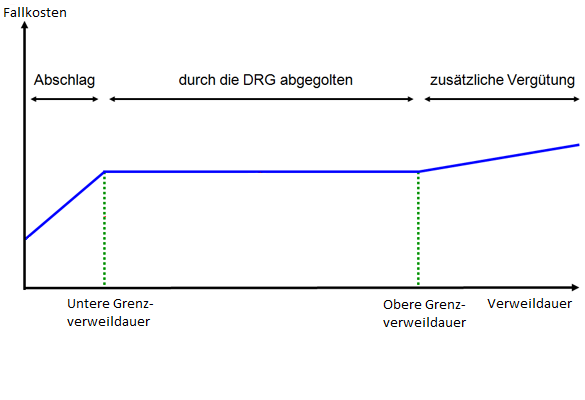
\includegraphics[width=0.8\textwidth]{./bilder/drg}
\caption{DRG-Fallkostenentwicklung (eigene Darstellung)} 
\label{fig:DRG} 
\end{figure}

Am Ende wird das resultierende Kostengewicht mit dem Basisfallwert multipliziert, um die Kosten des Krankenhausfalles zu bestimmen. Der Basisfallwert wird dabei j�hrlich f�r jedes Bundesland neu berechnet. Aktuell liegt dieser Wert zwischen 3.190,81 Euro und 3.311,98 Euro\footnote{Quelle: \url{http://www.gkv-spitzenverband.de/krankenversicherung/krankenhaeuser/budgetverhandlungen/bundesbasisfallwert/bundesbasisfallwert.jsp} (Stand 8.2.2015)}. Das System wird vom "`Institut f�r das Entgeltsystem im Krankenhaus"'\footnote{\url{www.g-drg.de} (Stand 8.2.2015)} (kurz InEK) gepflegt und weiterentwickelt. \\

Die w�hrend eines Krankenhausaufenthalts gestellten Diagnosen und die durchgef�hrten Prozeduren werden nach den medizinischen Klassifikationen ICD-10-GM und OPS kodiert. Das ICD-10-GM ist eine f�r Deutschland angepasste Version der "`internationalen statistischen Klassifikation der Krankheiten und verwandter Gesundheitsprobleme"'(kurz: ICD\footnote{Aufgrund des englischen Namens: "`International Statistical Classification of Diseases and Related Health Problems"'}). Der zugeh�rige Katalog wird vom "`deutschen Institut f�r Medizinische Dokumentation und Information"'\footnote{\url{www.dimdi.de}},kurz DIMDI, j�hrlich aktualisiert und angepasst. Er ist hierarchisch strukturiert und enth�lt 22 Krankheitskapitel, die sich in Gruppen, Kategorien und Subkategorien aufsplitten. Das DIMDI sch�tzt die Anzahl der Schl�sselnummern auf ca. 13.400.  Die j�hrlichen Anpassungen stellen auch eine besondere Herausforderung bei der Arbeit mit ICD-Schl�sseln dar. Es kann vorkommen, dass in zwei unterschiedlichen Jahren einem ICD-Schl�ssel unterschiedliche Diagnosen zugeordnet werden. Der Operationen- und Prozedurenschl�ssel (kurz: OPS) wird ebenfalls vom DIMDI gepflegt und ist die amtliche Klassifikation zum Verschl�sseln von Operationen, Prozeduren und allgemein medizinischen Ma�nahmen im station�ren Bereich und beim ambulanten Operieren. \\

Sowohl die DRG- als auch ICD-Informationen sind, in den Grunddaten, f�r jeden einzelnen Krankenhausfall aufgeschl�sselt. Es ist zu beachten, dass alle w�hrend eines Kranhausfalles gestellten Diagnosen erfasst werden. Das hei�t es k�nnen auch Diagnosen vorkommen, die mit der DRG nicht in Zusammenhang stehen\footnote{z.B. ein Herzinfarkt w�hrend einer Operation}. Die Datenstruktur der aufbereiteten Daten wird in folgendem Diagramm veranschaulicht:

\begin{figure}[htb]                     
\centering 
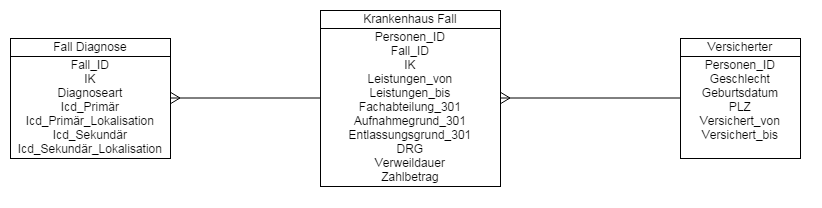
\includegraphics[width=0.8\textwidth]{./bilder/ER-Diagramm}
\caption{ER-Diagramm Datengrundlage} 
\label{fig:Datengrundlage} 
\end{figure}

\begin{enumerate}[label=(\roman{*})]
	\item \textbf{Versicherter:} In der ersten Tabelle sind Information zu den Versicherten hinterlegt. Neben Geschlecht und Geburtsdatum, gibt es auch Information �ber den Wohnort(Postleitzahl) und den Zeitraum in dem er versichert war. Letzteres ist wichtig, da nur w�hrend dieses Zeitraums Leistungsdaten �ber den entsprechenden Versicherten vorliegen. Als Prim�rschl�ssel wird in dieser Tabelle die Personen\_ID verwendet, wodurch dann auch eine Zuordnung zu den Krankenhaus Falldaten m�glich ist.\\

	\item \textbf{Krankenhaus\_Fall:} Ein Krankenhausfall umfasst alle Ma�nahmen, die von der Einweisung bis zu Entlassung eines Versicherten f�llig werden. In dieser Tabelle kommt ein zusammengesetzter Prim�rschl�ssel aus Fall\_ID und Institutionskennzeichen des Krankenhauses (IK) zum Einsatz \footnote{Das ist notwendig da jedes Krankenhaus die Fall\_ID selbst vergibt und es so vorkommt das zwei Krankenh�user dieselbe ID vergeben.}. F�r jeden Behandlungsfall gibt es Daten zum Zeitpunkt und Grund der Aufnahme und Analog f�r die Entlassung. Au�erdem wird die abgerechnete DRG und die damit verbundenen Kosten angegeben. 

	\item \textbf{Fall\_Diagnose:} Zu jedem Fall sind au�erdem die dazugeh�rigen Diagnosen hinterlegt. Diese k�nnen wieder �ber die Kombination aus Institutionskennzeichen und Fall\_ID zugeordnet werden. Die Diagnosen werden nach dem oben beschrieben ICD-Katalog codiert und in Haupt- und Nebendiagnosen unterteilt, durch das Feld Diagnoseart. Jeder Datensatz enth�lt eine Prim�re ICD zu der falls notwendig auch die Lokalisation angegeben wird. Das ist z.B. notwendig um zu spezifizieren, ob der linke oder der rechte Arm gebrochen ist. In einigen wenigen F�llen gibt es auch noch eine Sekund�re ICD.

\end{enumerate}

\subsection{Identifizierung von Unf�llen}

Eine Herausforderung dieser Arbeit war es, aus den sehr umfangreichen Abrechnungsdaten, die F�lle zu identifizieren, die als Unf�lle im Sinne des Kohorten-Modells interpretiert werden k�nnen. In diesem Zusammenhang sollte nochmal erw�hnt werden, dass alle F�lle die nicht �ber die in diesem Abschnitt beschrieben Methodik erfasst werden k�nnen, trotzdem bilanziell im Kohorten Modell erfasst sind. Diese werden dann der Phase regen Lebens zugeordnet und somit gehen keine Kosten verloren. \\

Das wichtigste Erkennungsmerkmal der Unf�lle ist, dass sie sich nicht ank�ndigen. Deshalb ist der Aufnahmegrund im Krankenhaus ein guter Indikator daf�r, ob der Patient mit �berweisung oder Termin aufgenommen wurde oder nicht. In den Daten ist der Aufnahmegrund entsprechend den gesetzlichen Vorgaben codiert\footnote{siehe Anhang \ref{sec:301}}. Die f�r uns relevanten Informationen sind in der 3. und 4. Stelle codiert. Die folgenden Tabelle liefert eine �bersicht der m�glichen Auspr�gungen und der relativen H�ufigkeiten in den Daten: \\

\begin{table}[H]
	\centering
	\begin{tabular}{|l|l|r|}
		\hline
		Code & Aufnahmegrund &	Anteil \\
		\hline
		01 & Normalfall & 56,704\% \\
		\hline
		07 & Notfall & 38,566\% \\
		\hline
		03 & Verkehrsunfall / Sportunfall / Sonstiger Unfall	& 0,105\% \\
		\hline
		02 & Arbeitsunfall / Wegeunfall / Berufskrankheit & 0,021\% \\
		\hline
		06 & Kriegsbesch�digten-Leiden / BVG-Leiden & 0,003\% \\
		\hline
		04 & Hinweis auf Einwirkung von �u�erer Gewalt	& 0,002\% \\
		\hline
		05 & frei (fr�her Hinweis auf Selbstmord / Selbstbesch�digung\footnote{Wird wegen Datenschutz nicht mehr codiert und ist f�r uns nicht relevant.})	& 0,001\% \\
		\hline
		\hline
			 &\textit{Keine Angabe (Feld nicht gef�llt)}	& 4,598\% \\
		\hline
	\end{tabular}
	\caption{Aufnahmegrund und relative H�ufigkeiten}
	\label{tbl:Aufnahme}
\end{table}

Mehr als die H�lfte der Krankenhausf�lle werden als Normalfall klassifiziert und kommen somit �ber eine �berweisung oder mit Termin ins Krankenhaus. Ein sehr kleiner Teil wird aufgrund einer Kriegsbesch�digung(06) behandelt oder aufgrund eines Gewaltverbrechens(04).  F�r uns interessant sind also die Notf�lle und die F�lle die tats�chlich als Unfall aufgenommen werden (02 und 03). Letztere machen leider nur einen sehr kleinen Teil aus, was auf die Natur der Daten zur�ckzuf�hren ist. Diese Schl�ssel werden nur vergeben, wenn es versicherungsrelevant ist. Damit konnten wir den Anteil der m�glich Unf�lle bereits auf ca. 40\% der Krankenhausf�lle einschr�nken. \\

Den n�chsten Anhaltspunkt liefert der Entlassungs- bzw. Verlegungsgrund. Allerdings gibt es 25 verschiedene Auspr�gungen und zus�tzlich die Information, ob der Versicherte arbeitsf�hig entlassen wurde\footnote{siehe Anhang \ref{sec:301}}. Deshalb erl�utern wir lediglich die interessanten F�lle, welche in der nachfolgenden Tabelle zusammengefasst sind. Die Anteile beziehen sich dabei bereits nur auf Notf�lle und Unf�lle:  \\

\begin{table}[H]
	\centering
	\begin{tabular}{|l|r|}
		\hline
		Entlassungsgrund &	Anteil \\
		\hline
		Behandlung beendet & 83,210\% \\
		\hline
		Tod oder Entlassung in ein Hospiz & 5,796\% \\
		\hline
		Entlassung in eine Pflegeeinrichtung	& 3,199\% \\
		\hline
		Entlassung in eine REHA-Einrichtung & 2,219\% \\
		\hline
		Sonstige & 5,575\% \\
		\hline
	\end{tabular}
	\caption{Entlassungsgrund und relative H�ufigkeiten f�r Not- und Unf�lle}
	\label{tbl:Entlassung}
\end{table} 

F�r den Gro�teil der Not- und Unf�lle, endet mit dem Krankenhausaufenthalt auch die Behandlung. Ein Teil der Patienten stirbt oder muss in ein Hospiz verlegt werden. Diese F�lle werden in der Pr�mortalit�tsphase des Kohorten-Modells erfasst und sind somit f�r die Singul�ren Ereignisse, nicht relevant. F�lle mit anschlie�ender Pflege sind f�r die Singul�ren Ereignisketten von Relevanz. Diese werden im n�chsten Kapitel behandelt. Unter Sonstige sind insbesondere die nicht trivialen F�lle zusammengefasst. Das bedeutet in erster Linie eine Verlegung oder eine Entlassungen aus abrechnungstechnischen Gr�nden. In diesen F�llen muss der weitere Verlauf aufw�ndig rekonstruiert werden, was nicht immer gelingt. Insbesondere bei einen Kassenwechsel des Patienten stehen die Information i.d.R. nicht zur Verf�gung. Hier muss dann abh�ngig vom jeweiligen Unfalltyp entschieden werden, ob sich der Aufwand lohnt. Gelingt die Rekonstruktion der Behandlungspfade, m�ssten die Kosten aller relevanten Anschlussbehandlung zu den Unfallkosten hinzugez�hlt werden. Gelingt dies nicht, d�rfen die F�lle trotzdem nicht vernachl�ssigt werden. Da allerdings keine Aussage �ber die Kosten getroffen werden kann, findet der Fall nur bei der Modellierung der Unfallwahrscheinlichkeit Beachtung, nicht aber bei der Modellierung der Kostenverteilung.\\

Nachdem die m�glichen Unf�lle aufgrund des Aufnahme und Entlassungsgrundes eingegrenzt wurden, sind in den Daten nur noch die DRG und ICD Informationen vorhanden. Zu jedem Fall gibt es eine DRG und mehrere Diagnosen, wobei eine davon als Hauptdiagnose ausgezeichnet wird. Das INeK definiert die Hauptdiagnose als "`Die Diagnose, die nach Analyse als diejenige festgestellt wurde, die haupts�chlich f�r die Veranlassung des station�ren Krankenhausaufenthaltes des Patienten verantwortlich ist."'\footnote{vgl. Kodierrichtlinien Seite 4 \url{http://www.g-drg.de/cms/content/view/full/5064}}. Deshalb kann die Hauptdiagnose verwendet werden, um verschiedene Unf�lle voneinander abzugrenzen. Es kommt aber vor, dass w�hrend der Behandlung andere Erkrankung entdeckt werden und dadurch die Hauptdiagnose am Ende f�r die DRG und damit f�r die Kosten, kaum eine Rolle spielt. An dieser Stelle sollte erw�hnt werden, dass ein Krankenhaus ein Unternehmen ist, welches darauf ausgerichtet ist Gewinn zu erwirtschaften. Deshalb besteht die Gefahr, dass Information ver�ndert werden um h�here Fallpauschalen zu kassieren oder um Patienten aufnehmen zu k�nnen, die eigentlich an andere Einrichtungen verwiesen werden m�ssten.\\

Aufgrund der Komplexit�t der m�glichen Krankenhausf�lle ist es schwierig eine allgemeine Vorgehensweise zu beschreiben, um die Unf�lle exakt abzugrenzen. Die vergeben Diagnosen liefern einen guten Anhaltspunkt daf�r, was mit dem Patienten passiert und warum er im Krankenhaus ist. Insbesondere ist dabei die Kategorie S00-T98:	"`Verletzungen, Vergiftungen und bestimmte andere Folgen �u�erer Ursachen"' hervorzuheben, da diese Diagnosen gut zu unserer Definition von Unf�llen passen. Eine Abgrenzung nur auf Basis der Diagnosen ist allerdings schwierig, da viele F�lle mehrere Diagnosen und  haben und wir sicherstellen m�ssen, dass es bei der Definition der Unfalltypen nicht zu �berschneidungen kommt. Au�erdem h�ngen die gestellten Diagnosen nicht immer mit der gew�hlten Behandlung zusammen und somit sind auch keine R�ckschl�sse auf die Kosten m�glich. Die DRG dr�ckt hingegen nur aus, welche Behandlung vom Krankenhaus abgerechnet wurde. Ein DRG deckt allerdings einen gro�en Bereich an F�llen ab und dabei auch F�lle, die wir nicht als Unf�lle definieren w�rden.\\

Zur weiteren Abgrenzung von Unf�llen ist also eine Kombination aus DRG und Diagnose n�tig. Diese lassen sich teilweise nur mit medizinischen Hintergrundwissen identifizieren. Der Vorteil des Kohorten-Modells ist es, dass unabh�ngig davon wie vollst�ndig man die Unf�lle abgrenzt keine Kosten verloren gehen. Die restlichen Kosten werden alle in der Phase regen Lebens erfasst. \\

F�r die Auswahl des Testfalls im n�chsten Abschnitt wurden die h�ufigsten Hauptdiagnosen betrachtet. Das sind Hypertonie, Herzinsuffizienz, Ohnmacht oder eine Gehirnersch�tterung. Hypertonie oder eine Herzinsuffizienz sind in unserem Sinne keine Unf�lle, da es h�ufig bereits im Vorfeld Anzeichen f�r eine solche Erkrankung gibt. Eine Ohnmacht kann dagegen sehr vielf�ltige Ursachen haben, wovon einige mit unserer Unfalldefinition konform sind und andere nicht. Die Gehirnersch�tterung ist dahingegen eine nachvollziehbare Unfalldiagnose und wurde deshalb f�r unser Anwendungsbeispiel ausgew�hlt. 

\subsection{Anwendung und Test des Poisson-Modells}

In diesem Abschnitt werden wir, am Beispiel vom Unfall Gehirnersch�tterung, den vorgestellten Poisson-Ansatz implementieren und bewerten. Dazu ist es notwendig eine saubere Datenbasis auszuw�hlen, auf der die notwendigen Parameter gesch�tzt werden k�nnen. Au�erdem werden wir eine Testmenge definieren, die sp�ter zur Bewertung des fertigen Modells verwendet wird. Es existieren Daten von drei Jahren (2009,2010 und 2011). Deshalb werden wir das erste Jahr (2009) f�r die Sch�tzung der Modellparameter verwenden und die anderen Beiden f�r den Test. Jedem Jahr ordnen wir alle Unf�lle zu, die in dem jeweiligen Jahr begonnen haben. Alle Kosten eine Falles, werden auf den Tag der Krankenhauseinweisung konzentriert, auch wenn sie in nachfolgende Jahre anfallen. \\

Im vorangegangenen Abschnitt haben wir bereits erl�utert, wie die Abrechnungsdaten nach Aufnahme und Entlassungsgrund gefiltert werden k�nnen, um die relevanten F�lle zu identifizieren. Dieselben Filter wurden auch verwendet, um die Grundtabelle mit allen potentiellen Unf�llen zu erstellen\footnote{siehe Anhang \ref{sec:scripts}}. Dazu wurde der MS SQL Server als Datenbank verwendet und die ben�tigten Abfragen per SQL formuliert. Anschlie�end wurden alle F�lle betrachtet, die als Hauptdiagnose die S06.0 "'Gehirnersch�tterung"' hatten, um zu untersuchen welche DRGs in diesen F�llen abgerechnet wurden. Die h�ufigste DRG (Anteil $97,5\%$) ist die B80Z: "`Andere Kopfverletzung"', also die Behandlung wegen einer Kopfverletzung. Es gab auch F�lle die mit der Diagnose Gehirnersch�tterung eingeliefert wurden und bei denen dann ein Herzschrittmacher eingesetzt wurde, was zu einer ganz anderen DRG gef�hrt hat. Daran zeigt sich weshalb die Kombination aus Diagnose und DRG wichtig f�r die Abgrenzung ist. F�r unseren Test beschr�nken wir uns deshalb auf alle F�lle die wegen einer Gehirnersch�tterung aufgenommen wurden und auch wegen einer Kopfverletzung behandelt wurden. \\

Neben den Fallinformationen ben�tigen wir au�erdem die Personeninformationen. In der entsprechenden Grundtabelle sind f�r jeden Versicherten mehrere Eintr�ge vorhanden. Jeder dieser Eintr�ge hat dabei dieselben Grundinformationen, wie Alter und Geschlecht, aber unterschiedliche Angaben zu dem Versicherungszeitraum. Um herauszufinden, ob ein Versicherter in einem bestimmten Zeitraum versichert war, m�ssen die einzelnen Zeitr�ume zusammengef�hrt werden. Da dies mit SQL sehr aufwendig ist, wurde ein JAVA Programm geschrieben, das diese Aufgabe erf�llt. Als Eingabe dienen die Personeninformationen und das Jahr, welches ausgewertet werden soll. Anschlie�end pr�ft das Programm f�r jeden Versicherten, welche Zeitintervalle in das beobachtete Jahr fallen und gibt die Anzahl der Tage aus, die der Versicherte in diesem Jahr bei der Kasse war. Zus�tzlich wird noch das Alter\footnote{Differenz aus betrachtetem Jahr und Geburtsjahr} des Versicherten im jeweiligen Jahr bestimmt. Diese Informationen werden dann im einem letzten Schritt an die Unfalldaten angespielt und ausgegeben. Die so erzeugte Grundtabelle bietet die Basis f�r das weitere Vorgehen.\\

Im ersten Schritt betrachten wir die Unfallwahrscheinlichkeit $\lambda$. Da ein Poisson-Prozess station�re Zuw�chse besitzt, k�nnen wir diese auf Basis der relativen H�ufigkeit in den historischen Daten sch�tzen. 
\begin{eqnarray*}
	\bar{\lambda} = \frac{\#\text{Unfall}}{\#\text{Versicherte}}.
\end{eqnarray*}
Dabei ist $\#\text{Unfall}$ in unserem Beispiel, die Anzahl alle Krankenhausf�lle, die in dem betrachteten Jahr(2009) begonnen haben. Dieser Wert wird durch die Anzahl aller Personen geteilt, die im betrachteten Zeitraum versichert waren. Das f�hrt zu der Frage wie Versicherte behandelt werden, die nicht �ber den gesamten betrachteten Zeitraum Versicherter waren. Diese d�rfen nicht ignoriert werden, da sonst evtl. relevante Informationen verloren gehen und das Modell verzerrt wird. Deshalb werden wir eine Gewichtung auf Basis der versicherten Tage vornehmen. Dementsprechend wird jemand, der nur 6 Monate versichert war, nur mit einem Gewicht von 0,5 in der Z�hlung ber�cksichtigt. Die Anzahl der Unf�lle wird dabei nicht gewichtet. Dementsprechend wird unterstellt das ein Versicherter, der nur ein halbes Jahr versichert war und in diesem Zeitraum einen Unfall hatte, dass dieser in der anderen Jahresh�lfte wieder einen Unfall hat. Da Unf�lle als seltene Ereignisse charakterisiert sind, f�hrt dieses Vorgehen also tendenziell zu einer �bersch�tzung der Unfallwahrscheinlichkeit. F�r unsere Testdaten ergibt sich in 2009 eine gesch�tzte Unfallwahrscheinlichkeit von $\bar{\lambda} = 0,189\%$ f�r das seltene Ereignis "`Gehirnersch�tterung"'. \\

Als n�chstes untersuchen wir, ob dieser Unfalltyp vom Alter und Geschlecht der Versicherten abh�ngt. Dazu unterteilen wir den Versichertenbestand in verschiedene Altersgruppen, die jeweils 5 Jahre umfassen. Die Neugeborenen sind dabei in einer extra Gruppe zusammengefasst, da diese in der ersten Phase des Kohorten-Modells betrachtet werden. Au�erdem bilden Versicherte die �lter sind als 90 eine Gruppe, da es in den hohen Altersbereichen nicht genug Versicherte gibt um allgemeine Aussagen ableiten zu k�nnen. Anschlie�end werden diese Gruppe noch Geschlecht getrennt. Wir bezeichnen diese Gruppen im Weiteren kurz als AGG f�r Alters- und Geschlechtsgruppe. Die folgende Grafik zeigt die Aufteilung der Grundgesamtheit in diese Gruppen.\\

\begin{figure}[htb]                     
\centering 
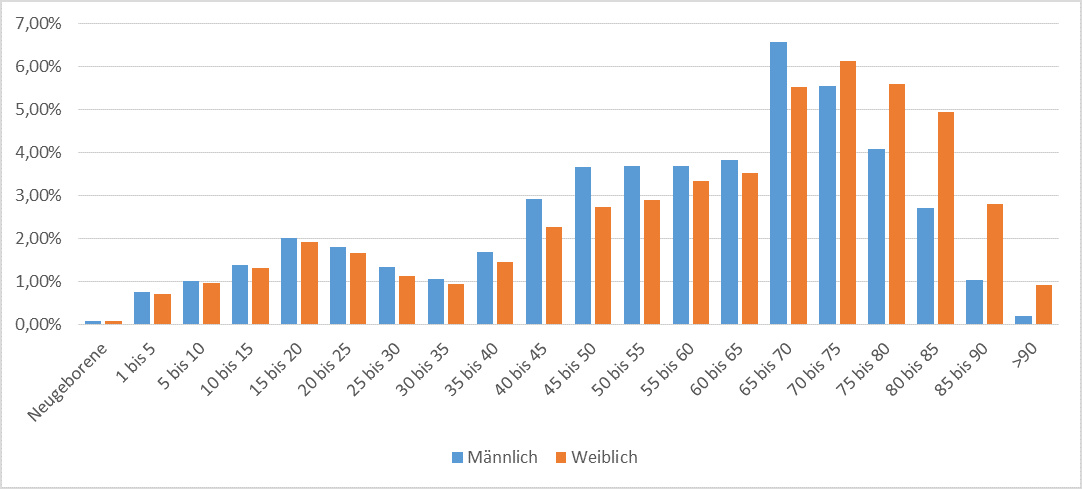
\includegraphics[width=0.8\textwidth]{./bilder/Diagramm_AnteileAGG}
\caption{Anteile in den Alters- und Geschlechtsgruppen} 
\label{fig:AnteileAGG} 
\end{figure}

Nun k�nnen wir f�r jede AGG die jeweiligen $\bar{\lambda}_{AGG}$ sch�tzen. Die folgende Grafik zeigt die relativen H�ufigkeiten f�r eine Gehirnersch�tterung in 2009, auf Basis der vorliegenden Daten. \\

\begin{figure}[htb]                     
\centering 
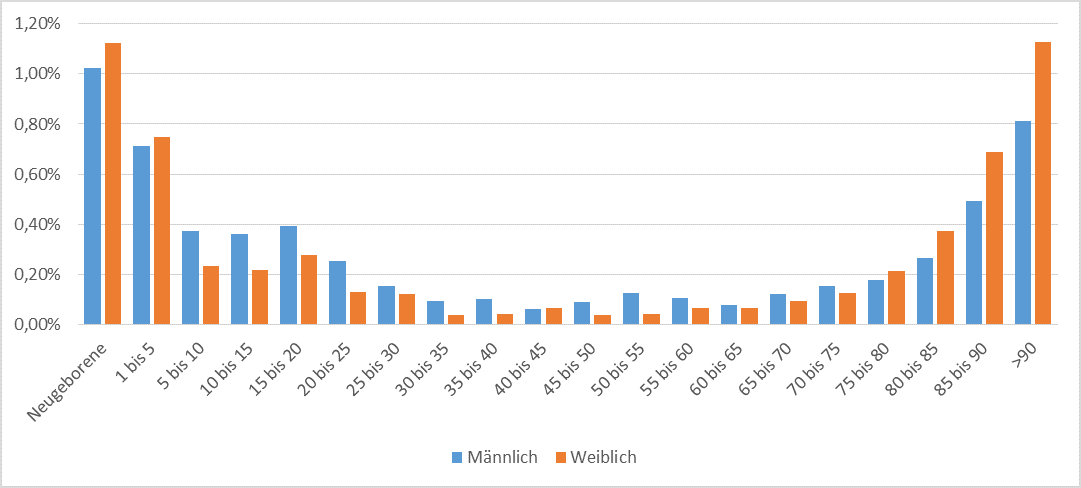
\includegraphics[width=0.8\textwidth]{./bilder/Diagramm_UnfallWs}
\caption{Gesch�tzte Unfallwahrscheinlichkeiten} 
\label{fig:UnfallWs} 
\end{figure}
Diese typische Badewannenkurve sieht man h�ufig im Zusammenhang mit Leistungen im Gesundheitswesen. Es ist klar zu sehen, dass im Vergleich zur durchschnittlichen Unfallwahrscheinlichkeit $\bar{\lambda}$, junge und alte Menschen zwei bis viermal so h�ufig wegen einer Gehirnersch�tterung behandelt wurden. Dahingegen liegt die H�ufigkeit im Altersbereich $30-65$, deutlich unter dem Durchschnitt.\\

Durch die sehr geringe Fallzahl bei Unf�llen, entsteht beim sch�tzen der Unfallwahrscheinlichkeiten ein hoher Standardfehler, also eine hohe mittlere Abweichung des gesch�tzten Parameters vom wahren Wert. Je kleiner die Altersgruppen werden, umso gr��er wird dieser. Da wir annehmen, dass die Anzahl der Unf�lle f�r einen Versicherten Poisson-Verteilt ist, ergibt sich der Standardfehler f�r eine AGG durch 
\begin{eqnarray*}
	\sigma_{\bar{\lambda}_{AGG}} = \sqrt{\frac{\bar{\lambda}_{AGG}}{\#\text{Versicherte}_{AGG}}}.
\end{eqnarray*}
Insbesondere in den schwach besetzten Gruppen ist deshalb die Genauigkeit der Sch�tzfunktion limitiert. Aus diesem Grund werden wir im Weiteren nur noch 3 Altersgruppen betrachten. Entsprechend den vorangegangen Beobachtungen unterteilen wir die Versicherten in Junge Leute, Erwachsene und Rentner. Diese Gruppen bilden dann auch die Grundlage f�r die Bewertung. Damit ergeben sich folgende Werte f�r die gesch�tzten Unfallwahrscheinlichkeiten und die entsprechenden Standardfehler.
\begin{table}[H]
	\centering
	\begin{tabular}{l|r|r|r|r}
		Gruppe & $\bar{\lambda}$ M�nner & $\bar{\lambda}$ Frauen & $\sigma$ M�nner & $\sigma$ Frauen\\
		\hline
		Junge Menschen(1-25 Jahre) & 0,3829\% & 0,2720\% & 0,0180\% & 0,0156\% \\
		\hline
		Erwachsene(26-65 Jahre) & 0,0973\% & 0,0585\% & 0,0051\% & 0,0043\%\\
		\hline
		Rentner(>65 Jahre) & 0,1867\% & 0,2820\% & 0,0074\% & 0,0080\%\\
	\end{tabular}
	\caption{�bersicht Unfallwahrscheinlichkeiten Gehirnersch�tterung}
	\label{tbl:overviewUnfallws}
\end{table}

Diese Unfallwahrscheinlichkeiten werden sp�ter dazu verwendet, die erwarteten Kosten eines Versicherten zu sch�tzen. Die Unterschiede zwischen den einzelnen Gruppen sind dabei deutlich zu erkennen.\\

Als n�chstes wollen wir die Kosten in den historischen Daten untersuchen, um f�r das Modell eine passende Kostenverteilung zu ermitteln. Zur Auswertung wurde in diesem Fall R\footnote{\url{http://www.r-project.org/}} gew�hlt. Das Programm ist in der Lage auch gr��ere Datenmengen schnell und zuverl�ssig zu untersuchen. Durch die Installation zus�tzlicher Bibliotheken, ist es au�erdem m�glich statistische Auswertungen und Test durchzuf�hren. Die folgende Grafiken zeigen zum Einen die Verteilung der Gesamtkosten und zum Anderen die Kosten pro Tag in 2009.

\begin{figure}[htb]
   \centering
      \subfloat[Gesamtkosten]{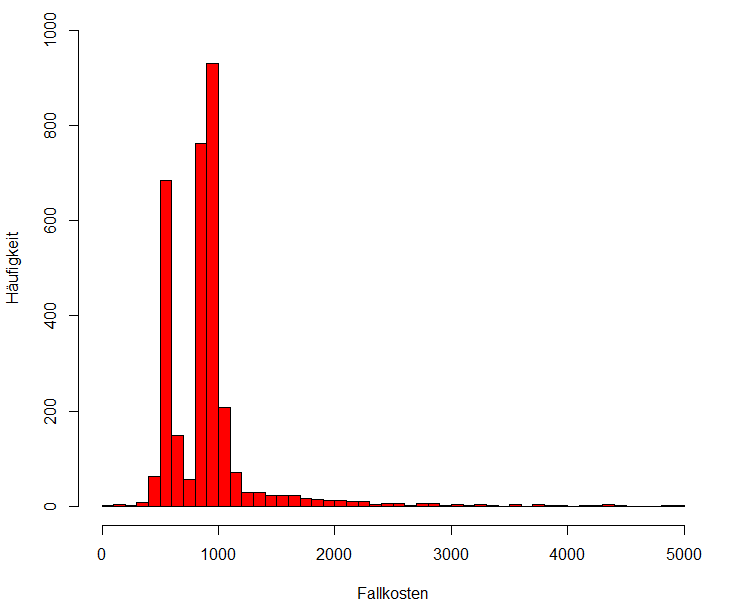
\includegraphics[width=0.45\textwidth]{./bilder/Kostenverteilung}}\qquad
      \subfloat[Kosten pro Tag]{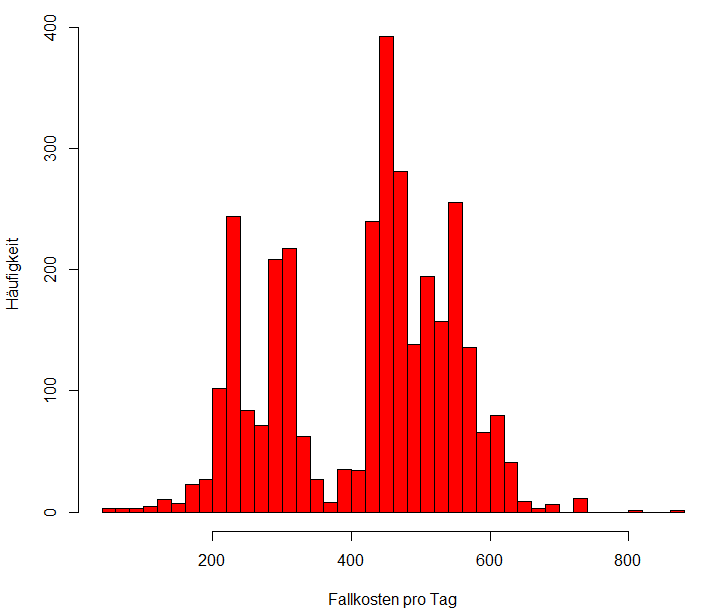
\includegraphics[width=0.45\textwidth]{./bilder/KostenProTag}}
   \caption{�bersicht Leistungskosten Gehirnersch�tterung}
	 \label{fig:overviewCost}
\end{figure}

In beiden Grafik ist deutlich zu erkennen, dass die Kostenverteilung zwei H�ufungspunkte besitzt. Das deutet auf eine �berlagerung von mindestens zwei Verteilungen hin. Die Ursache daf�r ist das Abrechnungssystem im Krankenhaus. Wie bereits beschrieben entsprechen die Kosten f�r einen Fall dem Produkt aus Kostengewicht und Basisfallwert. Der bundeslandspezifische Basisfallwert ist dabei innerhalb eines Jahres konstant. Das Kostengewicht h�ngt jedoch in erster Linie von der Verweildauer des Patienten im Krankenhaus ab. Der daraus resultierende Zusammenhang zwischen Kosten und Verweildauer l�sst sich f�r die DRG B80Z\footnote{Quelle: \url{http://drg.uni-muenster.de/index.php?option=com_drgsystematik&view=DRGSystematik&Itemid=49&mdc=01} (Stand: 8.2.2015)} wie folgt darstellen. 

\begin{figure}[H]                     
\centering 
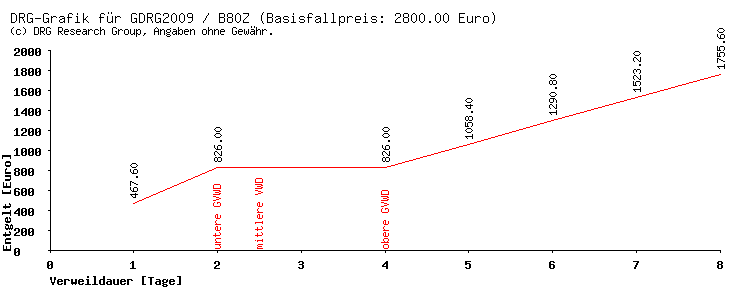
\includegraphics[width=0.8\textwidth]{./bilder/drgdiagrammB80Z}
\caption{DRG B80Z Kostenentwicklung} 
\label{fig:B80Z} 
\end{figure}

Das hei�t die untere Grenzverweildauer betr�gt zwei Tage und die obere Grenzverweildauer vier Tage. In diesem Zeitraum ist das Kostengewicht konstant und au�erhalb davon gibt es Zu- und Abschl�ge. Die Verteilung der Verweildauer ist dabei immer diskret, da das Abrechnungssystem nur ganze Tage ber�cksichtigt. Betrachten wir die Verweildauer f�r unsere F�lle, dann wird deutlich, dass die Mehrheit nur ein bis drei Tage im Krankenhaus aufgenommen wurden. Die mittlere Verweildauer betr�gt 1,8 Tage.

\begin{figure}[htb]                     
\centering 
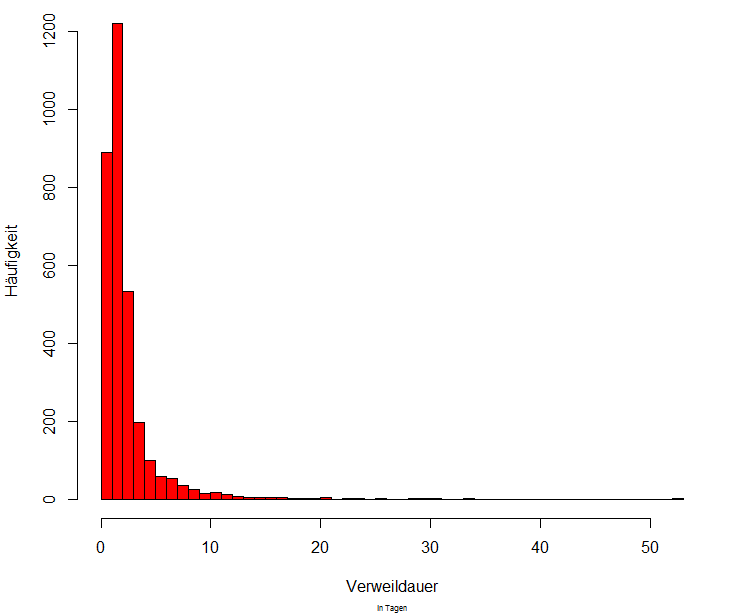
\includegraphics[width=0.7\textwidth]{./bilder/Verweildauer}
\caption{�bersicht Verweildauer Gehirnersch�tterung} 
\label{fig:verweildauer} 
\end{figure}

Durch dieses Zusammenhand zwischen der diskret verteilten Verweildauer und den Kosten f�r einen Fall, ist es sinnvoll die Kostenverteilung in drei Teile zu zerlegen. Jeweils eine Verteilung f�r die Zeit mit Abschl�gen auf das Kostengewicht (Verweildauer ein Tag), mit konstantem Kostengewicht (Verweildauer zwei bis vier Tage)und mit Zuschl�gen. Bezeichne $F_{A}, F_{K}$ und $F_{Z}$ jeweils die entsprechende Verteilungsfunktion und sei $V$ die Verweildauer, dann l�sst die Kostenverteilung wie folgt darstellen. 

\begin{eqnarray} \label{eq:kostenVerteilung}
	F_{Gesamt}(x) = \mathbb{P}(V \leq 1) F_{A}(x) + \mathbb{P}(V \leq 4 | V > 1) F_{K}(x) + \mathbb{P}(V > 4) F_{Z}(x)
\end{eqnarray}

Betrachten wir nun erneut die Verteilung der Kosten in den Daten, allerdings unterteilt nach Verweildauer, dann ergibt sich folgendes Bild. 

\begin{figure}[htb]
   \centering
      \subfloat[Verweildauer 1 Tag]{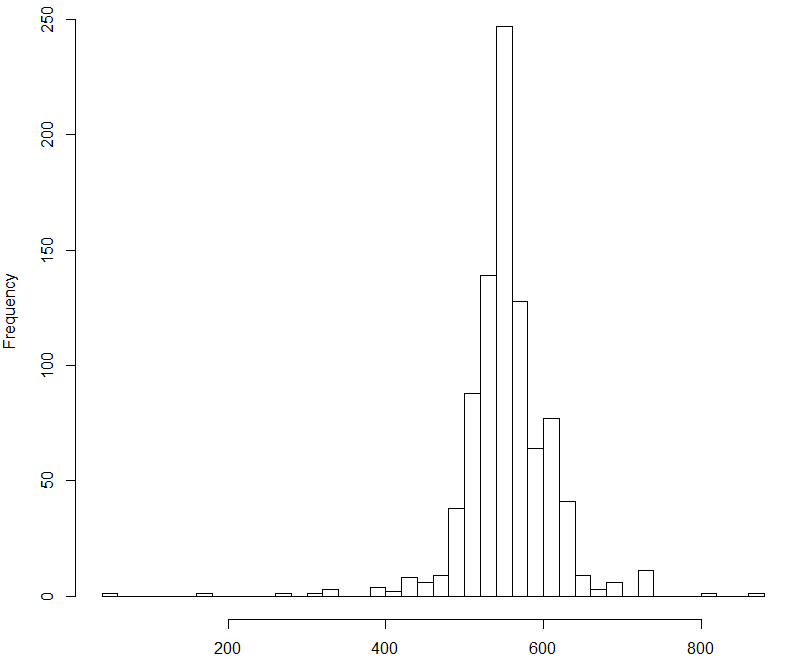
\includegraphics[width=0.45\textwidth]{./bilder/KostenUntereVWD}}\quad
      \subfloat[Verweildauer 2-4 Tage]{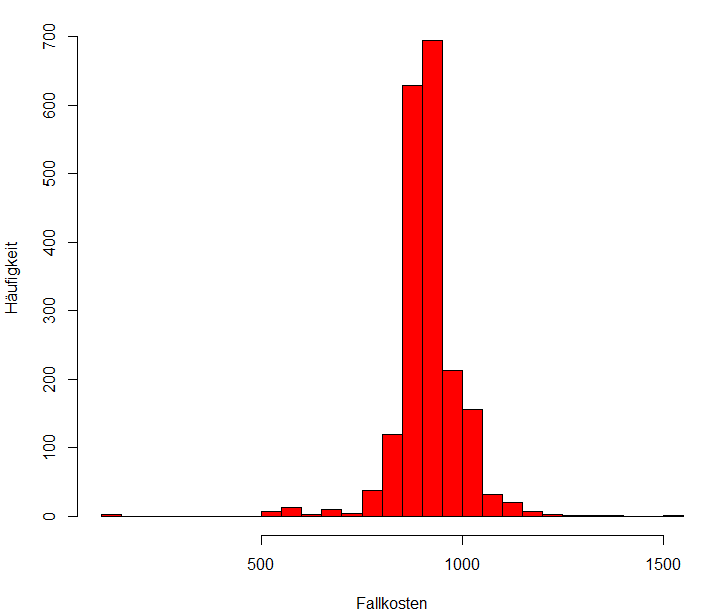
\includegraphics[width=0.45\textwidth]{./bilder/KostenMittlereVWD}}\quad
			\subfloat[Verweildauer >4 Tage]{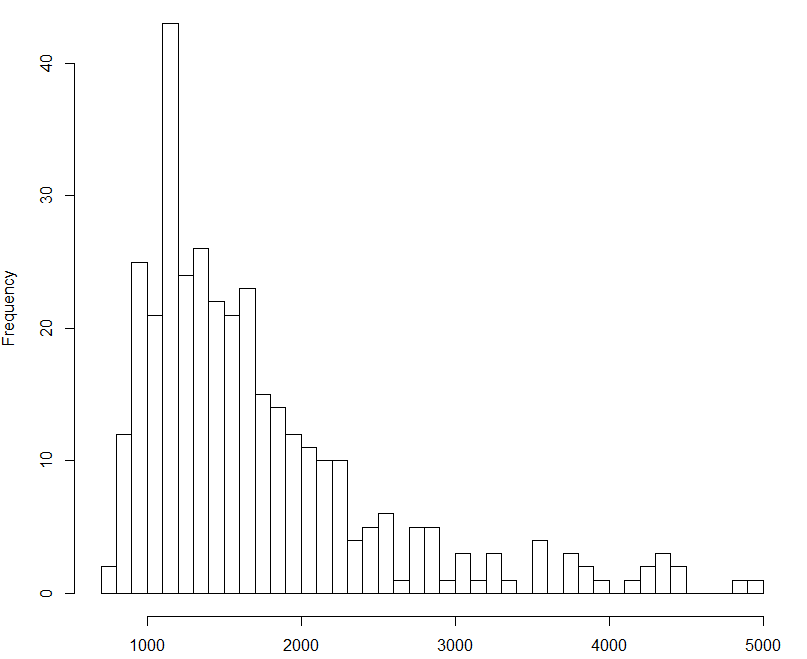
\includegraphics[width=0.45\textwidth]{./bilder/KostenHoheVWD}}
   \caption{�bersicht Leistungskosten unterteilt nach Verweildauer}
	 \label{fig:overviewCostVWE}
\end{figure}

Eine Approximation durch stetige Verteilung ist f�r keine der drei Verteilungen gelungen. Zum Testen wurde der Kolmogorow-Smirnow-Test verwendet und als m�gliche Verteilungen wurden Normalverteilung, Weibullverteilung, und im letzten Fall die Exponentialverteilung bzw. Gammaverteilung untersucht. In jedem Fall konnte die Nullhypothese bei einem Signifikanzniveau von 1\% verworfen werden. Aus diesem Grund verwenden wir im Weiteren die empirische Verteilung.\\

Der Erwartungswert der empirischen Kostenkostenverteilung, l�sst sich wieder mit Hilfe des Mittelwert-Sch�tzers bestimmen. Damit ergeben sich durchschnittliche Kosten in H�he von 922,85 Euro. Zusammen mit den gesch�tzten Unfallwahrscheinlichkeiten k�nnen wir somit das Risiko�quivalent f�r einen Versicherten bestimmen. Dieses ergibt sich als Summe der Barwerte, der erwarteten Kosten f�r alle Folgejahre, bis zum Eintritt in die Pr�mortalit�tsphase. Die erwarteten Kosten in einem Jahr entsprechen dem Erwartungswert des zusammengesetzten Poisson-Prozesses f�r dieses Jahr. Bezeichne $Y_t^{AGG}$ den zusammengesetzte Poisson-Prozess und $N_t^{AGG}$ den Poisson-Prozess f�r die Anzahl der Gehirnersch�tterungen, jeweils f�r einen Versicherten in der entsprechenden AGG. Weiterhin seinen ${X_i}$ die Kosten der i-ten Gehirnersch�tterung, dann gilt 
\begin{eqnarray} \label{eq:erwKostenGE}
	\mathbb{E}(Y_t^{AGG}) = \mathbb{E}(\sum_{i=1}^{N_t^{AGG}} X_i) = \lambda_{AGG}*t \mathbb{E}(X_i) = \lambda_{AGG}*t*922,85
\end{eqnarray}
Das hei�t z.B. die erwarteten Kosten f�r einen 30-j�hrigen Versicherten f�r das n�chste Jahr betragen rund 0,90 Euro.\\

F�r die Bewertung der Modellg�te werden wir untersuchen, wie sich die realen Kosten im Vergleich zu diesen Erwartungswerten entwickeln. Im ersten Schritt testen wir, ob sich die relevanten Modellparameter signifikant ver�ndert haben. Dazu f�hren wir einen Einstichproben-t-Test f�r die mittleren Fallkosten und einen gewichteten Einstichproben-t-Test f�r die alters- und geschlechtsabh�ngigen Unfallwahrscheinlichkeiten durch\footnote{Die entsprechenden Abfragen f�r R befinden sich im Anhang \ref{sec:scripts}.}. Die Nullhypothese ist dementsprechend, dass der Mittelwert der jeweiligen Daten aus 2010 gleich dem im Vorjahr gesch�tzten Modellparameter ist. Als Signifikanzniveau w�hlen wir 5\%.  Die folgende Tabelle zeigt eine �bersicht der Entwicklung der einzelnen Parameter und das Ergebnis des Tests.

\begin{table}[H]
	\centering
	\begin{tabular}{l|r|r|r}
		Parameter & Wert 2009 & Wert 2010 & p-Wert des t-Tests\\
		\hline
		Mittlere Fallkosten & 922,85 Euro & 922,07 Euro & 0,9254 \\
		\hline
		$\lambda$ Gesamt & 0,1890\% & 0,1891\% & 0,9838 \\
		\hline
		$\lambda$ Frauen 1-25 Jahre & 0,2720\% & 0,2897\% & 0,2971 \\
		\hline
		$\lambda$ Frauen 26-65 Jahre & 0,0585\% & 0,0631\% & 0,3356\\
		\hline
		$\lambda$ Frauen >65 Jahre & 0,2820\% & 0,2762\% & 0,4831\\
		\hline
		$\lambda$ M�nner 1-25 Jahre & 0,3829\% & 0,3574\% & 0,1751 \\
		\hline
		$\lambda$ M�nner 26-65 Jahre & 0,0973\% & 0,0930\% & 0,4090\\
		\hline
		$\lambda$ M�nner >65 Jahre & 0,1867\% & 0,2016\% & 0,0675\\
	\end{tabular}
	\caption{�bersicht Testergebnisse 2010}
	\label{tbl:overviewTestResults2010}
\end{table}

Da keiner der resultierenden p-Werte < 0,05 ist, konnte die Nullhypothese f�r keinen der getesteten Parameter verworfen werden. Dementsprechend scheint die Sch�tzung der Parameter erwartungstreu zu sein.\\

Um eine detailliertere Auswertung zu erm�glichen, werden wir zus�tzlich einen Simulationsansatz verfolgen. Anstatt einmal den gesamten Bestand auszuwerten, werden zuf�llig gezogene Stichproben untersucht. Da eine Stichprobe allein nur eine geringe Aussagekraft hat, werden wir entsprechend eines Monte-Carlo-Ansatzes, 10000 zuf�llige Stichproben analysieren. Die gesch�tzten und realen Kosten werden dann, f�r alle Versicherten in der Stichprobe, aufsummiert und verglichen. So erhalten wir ein Ma� f�r die Vorhersagegenauigkeit.\\

Zur Durchf�hrung der Stichprobenziehung und zur Berechnung der individuellen, erwarteten Unfallkosten, wurde wieder ein Java Programm erstellt. F�r jeden Versicherten werden dabei die erwarteten Kosten, entsprechend der Formel \ref{eq:erwKostenGE} bestimmt. Da wir $\lambda$ auf Basis der j�hrlichen Unfallrate gesch�tzt haben, entspricht der Zeitraum der Sch�tzung t, dem Anteil des Jahres, den der Versicherte bei der Kasse war. In jedem Durchlauf werden Stichproben mit einen Umfang von 100000 Versicherten gezogen. Anschlie�end werden die realen und die gesch�tzten Kosten aufsummiert und in eine separate Datei herausgeschrieben. Zur Auswertung der Ergebnisse kam wieder R zum Einsatz. \\

\begin{figure}[H]                     
\centering 
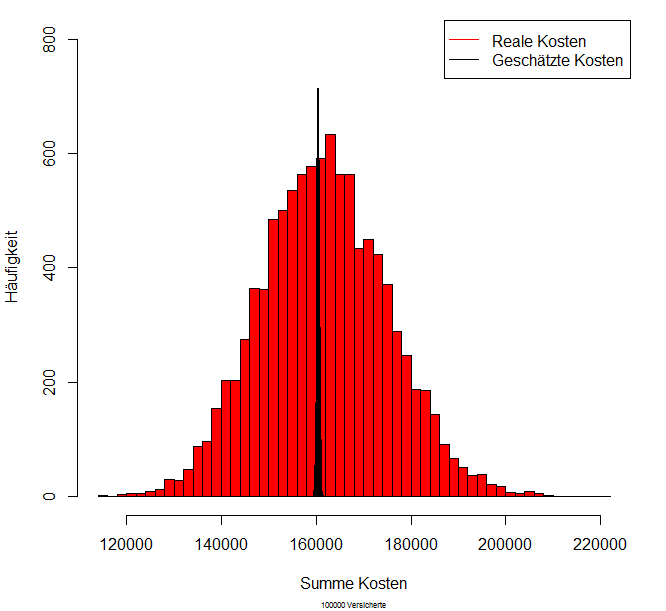
\includegraphics[width=0.7\textwidth]{./bilder/SimuResultHisto}
\caption{Ergebnis Simulation 2010} 
\label{fig:SimuResultHisto} 
\end{figure}

Aufgrund der geringen Varianz der Erwartungswertsch�tzung, sind die gesch�tzten kosten auf ein kleines Intervall konzentriert. Trotzdem ist gut zu sehen, dass die Mittelwerte der beiden Verteilungen sehr dicht beieinander liegen. F�r die realen Kosten ist dieser Wert 161695,80 Euro und f�r die gesch�tzten Kosten 160408,70 Euro. Das best�tigt die Ergebnisse des t-Test f�r die Modellparameter.\\

Der Vorteil des Simulationsansatzes ist, dass wir die Differenz zwischen realen und gesch�tzten Kosten untersuchen k�nnen, um ein Gef�hl f�r die Verteilung der Abweichung von den Erwarteten Kosten zu erhalten. Das folgende Histogramm zeigt die Verteilung der Kostendifferenzen in den 10000 Stichproben f�r 2010.\\

\begin{figure}[H]                     
\centering 
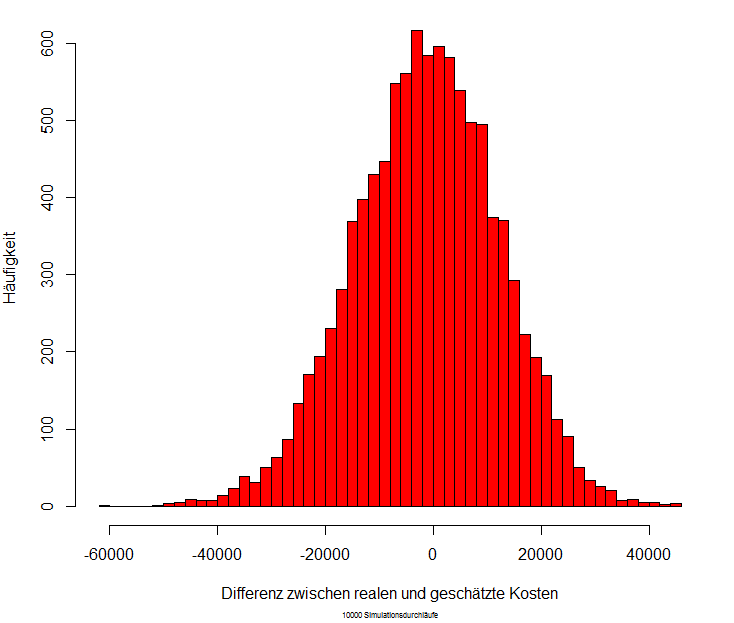
\includegraphics[width=0.7\textwidth]{./bilder/DifferenzKosten2010}
\caption{Differenzen der aufsummierten Kosten in 2010} 
\label{fig:Diff2010} 
\end{figure}

Der Mittelwert dieser Differenzen betr�gt -1287,04 Euro. Das hei�t wir untersch�tzen im Mittel die eintretenden Kosten f�r 2010 geringf�gig. Zur�ckzuf�hren ist dies auf eine leicht erh�hte Unfallrate in 2010. Obwohl die Differenzen normalverteilt aussehen, lie� sich dies nicht durch einen entsprechenden Test belegen. Ein angepasster Kolomogorov-Smirnow-Test (Lilliefors-Test) liefert einen p-Wert von 0,01326. Das hei�t bei einem Signifikanzniveau von 5\% muss die Nullhypothese, dass die Daten normalverteilt sind, verworfen werden. Trotzdem kann die empirische Verteilung dazu verwendet werden, Risikozuschl�ge zu bestimmen, damit wir die eintretenden Kosten nicht untersch�tzen.\\

Beispielsweise k�nnte der Risikozuschlag bestimmt werden, damit die Differenz aus realen Kosten und gesch�tzten Kosten in 95\% der F�lle positiv ist. Dazu betrachten wir im einfachsten Fall das 5\% Quantil der Verteilung in \ref{fig:Diff2010}: $Q_{0,05} = -23554,70$. Da jede Stichprobe 100000 Versicherte umfasst, w�rde ein einheitlicher Risikozuschlag von rund 24 Cent f�r jeden Versicherten ausreichen. Diese einfache Berechnung ist lediglich als Beispiel daf�r gedacht, wof�r die Verteilung der Abweichung verwendet werden kann. \\

Zusammenfassend l�sst sich sagen, dass der Poisson-Ansatz zur Modellierung der isolierten Ereignisse im Jahr 2010 stabile Ergebnisse produziert hat. \\

Nun betrachten wir das Jahr 2011 und untersuchen auch wieder die gesch�tzten Parameter mit Hilfe eines t-Test. 

\begin{table}[H]
	\centering
	\begin{tabular}{l|r|r|r}
		Parameter & Wert 2009 & Wert 2011 & p-Wert des t-Tests\\
		\hline
		Mittlere Fallkosten & 922,85 Euro & 933,43 Euro & 0,1382 \\
		\hline
		$\lambda$ Gesamt & 0,1890\% & 0,2056\% & 0,00002 \\
		\hline
		$\lambda$ Frauen 1-25 Jahre & 0,2720\% & 0,2941\% & 0,1909 \\
		\hline
		$\lambda$ Frauen 26-65 Jahre & 0,0585\% & 0,0611\% & 0,7179\\
		\hline
		$\lambda$ Frauen >65 Jahre & 0,2820\% & 0,3227\% & 0,00001\\
		\hline
		$\lambda$ M�nner 1-25 Jahre & 0,3829\% & 0,3882\% & 0,7801 \\
		\hline
		$\lambda$ M�nner 26-65 Jahre & 0,0973\% & 0,0954\% & 0,7221\\
		\hline
		$\lambda$ M�nner >65 Jahre & 0,1867\% & 0,2180\% & 0,0004\\
	\end{tabular}
	\caption{�bersicht Testergebnisse 2011}
	\label{tbl:overviewTestResults2011}
\end{table}
